
\section{概形可视化：相伴点与零因子}

模的\emph{\trAssociatedPoint}理论，是把\trSupport{}观念进一步精细化（\S4.1.7）。
\trAssociatedPoint{}将帮助我们理解并可视化\trNilpotent{}元，并把「\trRationalFunction」%
的观念推广到非\trIntegral{}的\trScheme。它们还有一些我们用不上的用途，例如经由它们
与\trPrimaryDecomposition{}（primary decomposition）的联系。而对我们来说，它们最大的用处或许在于帮助
我们理解并可视化（非）\trZerodivisor——后者将经由有效\trCartierDivisor{}与%
\trLineBundle、\trRegularSequence{}（regular sequences）、\trDepth{}与\textbf{\trCM}（Cohen--Macaulay）性等话题反复登场。

现在就来讨论\trAssociatedPoint{}并没有什么特别的理由，本节可以独立阅读，任君在闲暇时
再看。但这是一次练习几何可视化、并学一些有用代数的好机会。

\textbf{6.6.1.\ 动机。}\quad 图~\ref{fig:six-associated-points} 是某个\trScheme{} $X$ 的
一幅草图。我们看到两个\trConnectedComponent{}与三个\trIrreducibleComponent。$X$ 的诸%
\trIrreducibleComponent{}的\trDimension{}分别为 $2$、$1$ 与 $1$，尽管要等到第 12 章，
我们才能对「\trDimension」有确切的理解。两个\trConnectedComponent{}都是非\trReduced{}的。

在这幅图里还能多看出一点东西，本节将借助「\trAssociatedPoint」把它说精确。那个可约的%
\trConnectedComponent{}似乎在不同\trLocus{}上有着程度不同的非\trReduced{}行为。概形 $X$
有六个\trAssociatedPoint，它们是图中「可见」的那些\trIrreducible{}子集的\trGenericPoint。%
$X$ 上的一个函数是\trZerodivisor，只要它的\trZeroSet{}含有这六个\trIrreducible{}子簇中的
任何一个。

\begin{figure}[htbp]
\centering
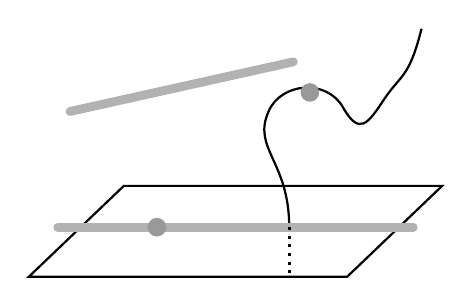
\begin{tikzpicture}[scale=1.05]
  \draw[line width=3.2pt,gray!60,line cap=round] (-2.6,1.9) -- (0.1,2.5);
  \draw[thick] (0.05,0.5) .. controls (0.05,1.3) and (-0.4,1.45) .. (-0.2,1.9)
    .. controls (-0.05,2.25) and (0.5,2.3) .. (0.7,1.95)
    .. controls (0.9,1.6) and (1.0,1.75) .. (1.2,2.05)
    .. controls (1.4,2.35) and (1.5,2.3) .. (1.65,2.9);
  \fill[gray!80] (0.3,2.13) circle (3.2pt);
  \draw[thick] (-3.1,-0.1) -- (0.75,-0.1) -- (1.9,1.0) -- (-1.95,1.0) -- cycle;
  \draw[line width=3.2pt,gray!60,line cap=round] (-2.75,0.5) -- (1.55,0.5);
  \fill[gray!80] (-1.55,0.5) circle (3.2pt);
  \draw[dotted,line width=1.1pt] (0.05,0.5) -- (0.05,-0.08);
\end{tikzpicture}
\caption{这个概形有六个\trAssociatedPoint，其中三个是\trEmbeddedPoint。一个函数只要在这
六个点中的任何一处消失，便是\trZerodivisor。（依原书手绘图重绘。）}%
\label{fig:six-associated-points}
\end{figure}

设 $M$ 是\trNoetherian{}环 $A$ 上的一个\trFinitelyGenerated{}\trModule。比如说，$M$ 也可以
就是 $A$ 自身。于是 $\Spec A$ 中有一些特殊的点，对理解 $M$ 而言尤为关键。它们就是 $M$ 的%
\emph{\trAssociatedPoint}（或者等价地说，$M$ 的\emph{\trAssociatedPrimeIdeal{}}（associated prime
ideals）——这两个术语我们将不加区分地混用）。作为动机，我们列出相伴点的亿十条性质，
把它们留给你依据本节其余部分所发展的理论去逐一验证。

在你阅读本节的过程中，不妨把
\[
M=A=k[x,y]/(y^2,\,xy)
\]
（\cref{fig:nonreduced-y2xy}）记在心头，作为贯穿本节的例子。

\textbf{6.6.2. 相伴点的亿十条性质。}\quad 下面是我们要证明的相伴点诸性质中的一部分。

相伴点只有有限多个：$\operatorname{Ass}_A M\subset\Spec A$。

$M$ 的\trSupport{}就是 $M$ 的诸\trAssociatedPoint{}的\trClosure：%
$\Supp M=\overline{\operatorname{Ass}_A M}$。$M$ 的任何一个\trSubmodule{}的\trSupport，是
$M$ 的诸\trAssociatedPoint{}中某个子集的\trClosure。$M$ 的任何一个元素的\trSupport，是
$M$ 的诸\trAssociatedPoint{}中某个子集的\trClosure。

$M$ 的诸\trAssociatedPoint，恰好就是对一切 $\mathrm{m}\in M$ 而言 $\Supp\mathrm{m}$ 的诸%
\trIrreducibleComponent{}的\trGenericPoint。$M$ 的诸\trAssociatedPoint，恰好是那些为%
\trIrreducible{}的诸 $\Supp\mathrm{m}$（$\mathrm{m}$ 跑遍 $M$ 的元素）的\trGenericPoint。%
$M$ 的\trAssociatedPrimeIdeal{}（associated primes），恰好就是那些作为 $M$ 中某个元素的\trAnnihilatorIdeal{}而出现的%
\trPrimeIdeal。

取「\trAssociatedPoint」与\trLocalization{}交换。因此这个观念本质上是几何的，这将使我们
得以（在 \S6.6.32 中）把它推广到局部诺特概形上的\trCoherentSheaf。

\trAssociatedPoint{}在正合列中的表现\emph{相当}好。例如，\trSubmodule{}的诸%
\trAssociatedPoint{}是原\trModule{}的诸\trAssociatedPoint{}的一个子集。

若 $I\subset A$ 是一个\trIdeal，则 $A/I$ 的\trAssociatedPrimeIdeal{} $\mathfrak{p}$，恰好就是那些使某个%
$\mathfrak{p}$-\trPrimary{}理想出现在 $I$ 的\trPrimaryDecomposition{}之中的 $\mathfrak{p}$。

我们将反复使用如下事实：\emph{$A$ 的一个元素是\trZerodivisor，当且仅当它在某个%
\trAssociatedPoint{}处消失}。

$A$ 的一个元素是\trNilpotent{}的，当且仅当它在每一个\trAssociatedPoint{}处消失。$\Spec A$
中使\trStalk{} $A_{\mathfrak{p}}$ 非\trReduced{}的那些点 $[\mathfrak{p}]$ 的\trLocus，是诸%
\trAssociatedPoint{}中某个子集的\trClosure。

一个处在另一个\trAssociatedPoint{}的\trClosure{}之中的\trAssociatedPoint，称为一个%
\emph{\trEmbeddedPoint}。若 $A$ 是\trReduced{}的，则 $\Spec A$ 没有\trEmbeddedPoint。%
$\mathbb{A}^n_k$ 中的\trHypersurface{}没有\trEmbeddedPoint。我们日后将看到：\trCompleteIntersection{}%
（complete intersections）没有\trEmbeddedPoint{}（\S26.2.7）。

$M$ 的元素由它们在诸\trAssociatedPoint{}处的\trLocalization{}所确定。相应的层
$\widetilde{M}$（\cref{ex:module-sheaf-on-base}）的\trSection{}由它们在诸%
\trAssociatedPoint{}处的\trGerm{}所确定。

以上讨论立即给出「局部诺特概形上的\trCoherentSheaf{}的\trAssociatedPoint」这一观念，
它带有这里描述的全部好性质。「局部诺特概形 $X$ 的\trAssociatedPoint」（不显式提及凝聚层）
一语，意思是「$\OO_X$ 的\trAssociatedPoint」；\textbf{\trEmbeddedPoint}亦同理。

我们现在就来建立这亿十条事实。

\textbf{6.6.3. 有关\trSupport{}观念的更多内容。}

$A$-\trModule{} $M$ 的\emph{\trAssociatedPoint}观念，是对\emph{\trSupport}观念的精细化
（在 $M$ 是\trNoetherian{}环 $A$ 上的\trFinitelyGenerated{}\trModule{}的情形）。（在下文
中，除非必要，我们不对 $A$ 是\trNoetherian{}的或 $M$ 是\trFinitelyGenerated{}的作任何
假设。）为作好铺垫，回忆（\S4.1.7）：$\mathrm{m}\in M$ 的\emph{\trSupport}
\[
\Supp\mathrm{m}=\{[\mathfrak{p}]\in\Spec A\ :\ \mathrm{m}_{\mathfrak{p}}\neq 0\}
\]
是一个\trClosedSubset，从而形如某个 $I$ 的 $V(I)$。练习~6.6.A 将给出「最佳的这个」$I$。
定义 $A$-\trModule{} $M$ 中元素 $\mathrm{m}$ 的\textbf{\trAnnihilatorIdeal{}}（annihilator ideal）
$\operatorname{Ann}_A\mathrm{m}\subset A$ 为：
\[
\operatorname{Ann}_A\mathrm{m}:=\{a\in A\ :\ a\mathrm{m}=0\}
  =\ker\bigl(A\xrightarrow{\times\mathrm{m}}M\bigr).
\]
当下标 $A$ 由上下文自明时，便略去不写。

\textbf{6.6.A.（轻松的重要练习）}\quad 证明：$\Supp\mathrm{m}=V(\operatorname{Ann}\mathrm{m})$。

回忆（\cref{thm:support-of-sheaf}）
\[
\Supp\widetilde{M}=\{[\mathfrak{p}]\in\Spec A\ :\ \widetilde{M}_{\mathfrak{p}}\neq 0\},
\]
以及与之类似的、\emph{\trModule{} $M$ 的\trSupport}的\cref{thm:support-of-module}：
\begin{equation*}\tag{6.6.3.1}\label{eq:supp-module-definition}
\Supp M:=\{[\mathfrak{p}]\in\Spec A\ :\ M_{\mathfrak{p}}\neq 0\},
\end{equation*}
于是 $\Supp M=\Supp\widetilde{M}$。若 $M$ 是由 $\mathrm{m}\in M$ 生成的主模（principal
module），则
\[
\Supp M=\Supp A\mathrm{m}=\Supp\mathrm{m}=V(\operatorname{Ann}\mathrm{m}).
\]

\trSupport{}与\trAssociatedPoint{}这两个观念在正合列中、以及在\trLocalization{}之下都有
良好的表现。我们现在就开始解释这一点。

\textbf{6.6.4.}\ \emph{\trSupport{}观念在正合列中表现良好。}

\textbf{6.6.B.（练习）}\quad 设 $0\to M'\to M\to M''\to 0$ 是 $A$-\trModule{}的一个%
\trShortExactSequence。

(a)~证明：$\Supp M=\Supp M'\cup\Supp M''$。

(b)~证明：若 $M$ 是\trFinitelyGenerated{}的\trModule，则 $\Supp M$ 是 $\Spec A$ 的一个%
\trClosedSubset。（提示：对生成元的个数作归纳。）

警示：一般地，$\Supp M$ 未必是闭的；考虑 $A=\mathbb{Z}$ 与
$M=\bigoplus_{\mathfrak{p}}\mathbb{Z}/(\mathfrak{p})$（对素数 $\mathfrak{p}$ 取直和）。

\textbf{6.6.C.（练习）}\quad 设 $M$ 是一个\trFinitelyGenerated{}的 $A$-\trModule，$x\in A$
在 $\Supp M$ 的所有点处取值均为 $0$，也就是说，$x$ 含于 $M$ 受支撑的每一个\trPrimeIdeal{}
之中。证明：$x$ 的某个幂 $x^n$ 零化 $M$ 的每一个元素。（提示：零化一组生成元。）

\textbf{6.6.D.（练习；将于 \S18.6 中使用）}\quad 设 $M$ 是一个\trFinitelyGenerated{}的
$A$-\trModule，$x\in A$。证明：$\Supp(M/xM)=(\Supp M)\cap V(x)$。这里 $M/xM$ 由正合列
\[
M\xrightarrow{\times x}M\longrightarrow M/xM\longrightarrow 0
\]
所定义。

\textbf{6.6.5.}\ \emph{\trhDefinition{}：\trAssociatedPoint{}与\trAssociatedPrimeIdeal{}。}

定义 $A$-\trModule{} $M$ 的\textbf{\trAssociatedPrimeIdeal{}}（associated prime ideals）为 $A$ 的形如
$\operatorname{Ann}_A(\mathrm{m})$（$\mathrm{m}\in M$）的那些\emph{\trPrimeIdeal}。定义
$M$ 的\textbf{\trAssociatedPoint}为 $\Spec A$ 中与之相应的那些点；「\trAssociatedPoint」%
与「\trAssociatedPrimeIdeal{}」这两个术语我们不加区分地混用。诸\trAssociatedPoint{}所成之集记作
$\operatorname{Ass}_A M\subset\Spec A$，下标 $A$ 在由上下文自明时省去。（为帮助记住定义
与记号，有人把它们称作 \emph{assassins}（刺客），因为它们正是那批能够毫不留情、毫无
悔意地零化\trModule{}中元素的素理想\footnote{译注：双关语——记号 $\operatorname{Ass}$
恰是「assassins」一词的后半截，而「assassinate」（行刺）又与「annihilate」（零化）音近。}。）
不过我们不会使用这个名称。

\textbf{6.6.6.}\quad 环 $A$ 的\textbf{\trAssociatedPrimeIdeal{}}（associated primes），就是把 $A$ 看作一个
$A$-\trModule{}（即取 $M=A$）时的\trAssociatedPrimeIdeal{}。

\textbf{6.6.E.（容易的练习：\trIntegralDomain{}的\trAssociatedPoint）}\quad 若 $A$ 是一个%
\trIntegralDomain，证明：$\operatorname{Ass}A=\{[(0)]\}$——零理想是唯一的\trAssociatedPrimeIdeal{}。

\textbf{6.6.F.（练习：\trHypersurface{}的\trAssociatedPoint）}\quad 给定
$f\in k[x_1,\dots,x_n]$，证明：$k[x_1,\dots,x_n]/(f)$ 的\trAssociatedPrimeIdeal{}，恰是那些由 $f$ 的素因子
生成的主理想。（你的论证将更一般地适用于任何 $f\in A$，其中 $A$ 是一个\trUFD。）

\textbf{6.6.7.}\ \emph{「$[\mathfrak{p}]\in\operatorname{Ass}_A(M)$ 当且仅当存在 $A$-%
\trModule{}的\trInclusionMap{} $A/\mathfrak{p}\hookrightarrow M$」这一观察将是必不可少
的。}下一个练习或许能把这一点敲实。

\textbf{6.6.G.（练习）}

(a)~设 $M'\subset M$。证明：$\operatorname{Ass}M'\subset\operatorname{Ass}M$。（「%
\trSupport」的相应陈述隐含在练习~6.6.B(a) 中。）

(b)~证明：$\operatorname{Ass}M\subset\Supp M$。

若 $M$ 是\trFinitelyGenerated{}的，则 $\Supp M$ 是闭的（练习~6.6.B），于是
$\overline{\operatorname{Ass}M}\subset\Supp M$。当 $A$ 是\trNoetherian{}的时，等号将在
命题~6.6.24 中证得。

\textbf{6.6.8. \trNoetherian{}环上的非零\trModule{}有\trAssociatedPoint。}

设 $\mathrm{m}$ 是 $A$-\trModule{} $M$ 的一个非零元素。注意：对 $\mathrm{m}$ 的任何非零
倍元 $x\mathrm{m}$，有 $\operatorname{Ann}\mathrm{m}\subseteq\operatorname{Ann}x\mathrm{m}%
\subsetneq A$。

\textbf{6.6.H.（练习）}\quad 设 $A$ 是\trNoetherian{}的。证明：存在某个倍元
$\mathrm{n}=x\mathrm{m}$，使得 $\mathrm{n}$ 的\emph{任何}满足 $\mathrm{yn}\neq 0$ 的非零
倍元 $y\mathrm{n}$ 都有 $\operatorname{Ann}y\mathrm{n}=\operatorname{Ann}\mathrm{n}$。

\textbf{6.6.9.\ \trhProposition。}\ ——\ \emph{沿用上一练习的记号，则
$\operatorname{Ann}\mathrm{n}$ 是一个\trPrimeIdeal。}

\emph{证明。}\ 设 $ab\in\operatorname{Ann}\mathrm{n}$，则 $ab\mathrm{n}=0$。于是要么
$b\mathrm{n}=0$（此时 $b\in\operatorname{Ann}\mathrm{n}$），要么
$a\in\operatorname{Ann}b\mathrm{n}=\operatorname{Ann}\mathrm{n}$。\hfill$\square$

于是我们便证明了下面的结论。

\textbf{6.6.10.\ \trhProposition{}（\trNoetherian{}环上的非零\trModule{}有\trAssociatedPrimeIdeal{}）。}\ ——\ %
\emph{若 $M$ 是\trNoetherian{}环 $A$ 上的一个非零\trModule，则 $\operatorname{Ass}_A M$
非空。更确切地说，对 $M$ 中任何 $\mathrm{m}\neq 0$，存在一个包含
$\operatorname{Ann}\mathrm{m}$ 的\trAssociatedPrimeIdeal{} $\mathfrak{p}$，并且对某个 $x\in A$ 有
$\mathfrak{p}=\operatorname{Ann}x\mathrm{m}$。}

\textbf{6.6.11. 在\trAssociatedPrimeIdeal{}处取\trLocalization。}

回忆一个有用的事实：$M\to\prod_{\mathfrak{p}\in\Spec A}M_{\mathfrak{p}}$ 是%
\trInjectiveMap{}（\cref{ex:module-to-product-localizations}）。我们眼下的处境还要好得多：
可以只对\emph{\trAssociatedPrimeIdeal{}}处的局部化取积。

\textbf{6.6.I.（练习）}\quad 设 $M$ 是\trNoetherian{}环 $A$ 上的一个\trModule。证明：
自然映射
\begin{equation*}\tag{6.6.11.1}\label{eq:ass-product-injection}
M\longrightarrow\prod_{\mathfrak{p}\in\operatorname{Ass}M}M_{\mathfrak{p}}
\end{equation*}
是\trInjectiveMap。提示：若\trKernel{} $K$ 非零，则 $K$ 有一个\trAssociatedPrimeIdeal{} $\mathfrak{p}$，它是
某个 $\mathrm{m}\in K\subset M$ 的\trAnnihilatorIdeal{}，而 $\mathrm{m}$ 在 $M_{\mathfrak{p}}$ 中非零。

显然，在 \eqref{eq:ass-product-injection} 中只需取诸\trAssociatedPrimeIdeal{}中的那些极大者。

\textbf{6.6.12. \trZerodivisor{}＝\trAssociatedPrimeIdeal{}的元素。}

\textbf{6.6.13.\ \trhProposition。}\ ——\ \emph{设 $f\in A$，$A$ 为\trNoetherian{}环。则
$f$ 是 $M$ 上的\trZerodivisor，当且仅当 $f$ 在 $M$ 的某个\trAssociatedPoint{}处消失。
翻译过来：\trZerodivisor{}之集是诸\trAssociatedPrimeIdeal{}的并。}

我们再一次只需诸\trAssociatedPrimeIdeal{}中的极大者。例如，若 $(A,\mathfrak{m})$ 是一个\trLocalRing，则
$\mathfrak{m}$ 是一个\trAssociatedPrimeIdeal{}，当且仅当 $\mathfrak{m}$ 的每一个元素都是\trZerodivisor。

\emph{证明。}\ 设 $f$ 在 $M$ 的某个\trAssociatedPoint{} $[\mathfrak{p}]$ 处消失。取
$\mathrm{m}$ 使 $\operatorname{Ann}\mathrm{m}=\mathfrak{p}$。则 $f\mathrm{m}=0$ 而
$\mathrm{m}\neq 0$，故 $f$ 是\trZerodivisor。

反之，若 $f$ 不在任何\trAssociatedPoint{}处消失，考虑交换图
\[
\begin{tikzcd}
M \ar[r,hook] \ar[d,"\times f"'] & \prod\limits_{\mathfrak{p}\in\operatorname{Ass}M}M_{\mathfrak{p}} \ar[d,"\times f"] \\
M \ar[r,hook] & \prod\limits_{\mathfrak{p}\in\operatorname{Ass}M}M_{\mathfrak{p}},
\end{tikzcd}
\]
其中的两行正是 \eqref{eq:ass-product-injection} 中的映射。右边的竖直箭头（乘以 $f$）由
假设是\trInjectiveMap，故左边的竖直箭头也必是\trInjectiveMap。\hfill$\square$

\textbf{6.6.14. \trAssociatedPoint{}在正合列中的表现\emph{相当}好。}

\textbf{6.6.15.\ \trhProposition。}\ ——\ \emph{设
\begin{equation*}\tag{6.6.15.1}\label{eq:ses-ass-context}
0\longrightarrow M'\longrightarrow M\longrightarrow M''\longrightarrow 0
\end{equation*}
是 $A$-\trModule{}的一个\trShortExactSequence。则
\begin{equation*}\tag{6.6.15.2}\label{eq:ass-inclusions-ses}
\operatorname{Ass}M'\subset\operatorname{Ass}M\subset\operatorname{Ass}M'\cup\operatorname{Ass}M''.
\end{equation*}}

我们来到了本节的第一个复杂证明。

\emph{证明。}\ \eqref{eq:ass-inclusions-ses} 的第一个包含关系已在练习~6.6.G(a) 中证得。

接下来设 $[\mathfrak{p}]\in\operatorname{Ass}M$，于是存在某个 $\mathrm{m}\in M$ 使
$\operatorname{Ann}\mathrm{m}=\mathfrak{p}$。我们希望找到一个\trIsomorphic{}于
$A/\mathfrak{p}$ 的、含于 $M'$ 或 $M''$ 的\trSubmodule。倘若本命题为真，我们就会期望在
「\eqref{eq:ses-ass-context} 的由 $\mathrm{m}$ 张成的那部分」中找到这样一个\trSubmodule。
于是我们转而考虑正合列
\[
0\longrightarrow A\mathrm{m}\cap M'\longrightarrow A\mathrm{m}
  \longrightarrow A\mathrm{m}/(A\mathrm{m}\cap M')\longrightarrow 0,
\]
注意这里出现的三个\trModule{}都是 \eqref{eq:ses-ass-context} 中相应\trModule{}的%
\trSubmodule。所以，由练习~6.6.G(a)，只须在这种「特殊情形」中证明本结论即可；而它可以
改写为
\[
0\longrightarrow I/\mathfrak{p}\longrightarrow A/\mathfrak{p}\longrightarrow A/I
  \longrightarrow 0,
\]
其中 $I$ 是把 $\mathrm{m}$ 视为\trModule{} $A\mathrm{m}/(A\mathrm{m}\cap M')$ 的元素时
的\trAnnihilatorIdeal{}。为方便起见，令 $B=A/\mathfrak{p}$（一个\trIntegralDomain），于是我们把这个
正合列进一步改写为下图的上行：
\[
\begin{tikzcd}
0 \ar[r] & J \ar[r] \ar[d,hook] & B \ar[r] \ar[d,hook] & B/J \ar[r] \ar[d,hook] & 0 \\
0 \ar[r] & M' \ar[r] & M \ar[r] & M'' \ar[r] & 0.
\end{tikzcd}
\]
现在把这一行 $B$-\trModule{}在 $(0)\subset B$ 处局部化，它便成为分式域 $K(B)$ 上%
\trVectorSpace{}的一个正合列，且中央元素是一维的：
\[
0\longrightarrow J\otimes K(B)\longrightarrow K(B)
  \longrightarrow(B/J)\otimes K(B)\longrightarrow 0.
\]
于是 $J\otimes K(B)$ 与 $(B/J)\otimes K(B)$ 这两端之一必有一个非零元素，它（把我们的
论证逆向追踪回去）给出 $M'$ 或 $M''$ 的一个元素，其\trAnnihilatorIdeal{}恰为 $\mathfrak{p}$。%
\hfill$\square$

\textbf{6.6.16.}\ \emph{警示性例子。}\quad $\mathbb{Z}$-\trModule{}的\trShortExactSequence
\[
0\longrightarrow\mathbb{Z}\xrightarrow{\times 2}\mathbb{Z}
  \longrightarrow\mathbb{Z}/2\longrightarrow 0
\]
（连同容易的练习~6.6.E）表明：$\operatorname{Ass}M=\operatorname{Ass}M'\cup\operatorname{Ass}M''$
并不总是成立。然而，有时我们仍能保证 $M''$ 的某些\trAssociatedPrimeIdeal{}提升为 $M$ 的\trAssociatedPrimeIdeal{}，届时将在
\S6.6.20 中看到。

\textbf{6.6.17. \trNoetherian{}环上的\trFinitelyGenerated{}\trModule{}只有有限多个%
\trAssociatedPoint{}／\trAssociatedPrimeIdeal{}。}

\textbf{6.6.J.（重要练习）}\quad 设 $M$ 是\trNoetherian{}环 $A$ 上的一个\trFinitelyGenerated{}%
\trModule。证明：$M$ 有一条（有限的）滤过（filtration）
\begin{equation*}\tag{6.6.17.1}\label{eq:filtration-quotient-primes}
0=M_0\subset M_1\subset\cdots\subset M_n=M,
\end{equation*}
其中对某个\trPrimeIdeal{} $\mathfrak{p}_i$ 有 $M_{i+1}/M_i\cong A/\mathfrak{p}_i$。
提示：借助命题~6.6.10，从左到右归纳地搭建 \eqref{eq:filtration-quotient-primes}，并证明
该过程终会终止。

\textbf{6.6.K.（练习）}\quad 设 $A$-\trModule{} $M$ 有一条有限滤过%
\eqref{eq:filtration-quotient-primes}，且不对\trFinitelyGenerated{}性或\trNoetherian{}性
作任何假设。证明：$M$ 的每一个\trAssociatedPrimeIdeal{}都作为诸 $\mathfrak{p}_i$ 之一出现。特别地，在这个
假设下（例如，若 $M$ 是\trNoetherian{}环上的\trFinitelyGenerated{}\trModule），$M$ 只有%
\emph{有限多个}\trAssociatedPoint{}／\trAssociatedPrimeIdeal{}。（提示：练习~6.6.E 与命题~6.6.15。）

\textbf{6.6.18.}\ \emph{警示：非相伴的素理想可能不可避免地出现在%
\eqref{eq:filtration-quotient-primes} 的诸商之中。}\quad 例子~6.6.16 表明，非相伴的素理想
可能出现在 \eqref{eq:filtration-quotient-primes} 的诸商之中，尽管在那样的情形里，缘由只是
滤过选得不明智。但更好的选择并不总能补救这一问题：

\textbf{6.6.L.（练习）}\quad 考虑环 $A=k[x,y]$ 上的\trModule{} $M=(x,y)\subset A$。证明：
$M$ 的\emph{任何}滤过 \eqref{eq:filtration-quotient-primes} 都含有某个商 $A/\mathfrak{p}_i$，
其中 $\mathfrak{p}_i$ \emph{不是}\trAssociatedPrimeIdeal{}。

\textbf{6.6.19.}\ \emph{\trhRemark{}。}\quad 然而，并非满盘皆输：练习~6.6.P 将证明，对
$M$ 的任何滤过 \eqref{eq:filtration-quotient-primes} 中的任何商 $A/\mathfrak{p}_i$，
$\mathfrak{p}_i$ 必\emph{包含} $M$ 的一个\trAssociatedPrimeIdeal{}。

\textbf{6.6.20. \trAssociatedPoint{}在正合列中的表现\emph{相当}好（续）。}

\textbf{6.6.21.\ \trhProposition。}\ ——\ \emph{设 $A$ 是\trNoetherian{}环。我们继续考虑
$A$-\trModule{}的\trShortExactSequence}
\[
0\longrightarrow M'\longrightarrow M\longrightarrow M''\longrightarrow 0
\]
\emph{设 $\mathfrak{p}\in\operatorname{Ass}M''$，但 $\mathfrak{p}\notin\Supp M'$（这是比
$\mathfrak{p}\notin\operatorname{Ass}M'$ 更强的假设）。则 $\mathfrak{p}\in\operatorname{Ass}M$。}

我们来到了本节的第二个复杂证明。

\emph{证明。}\ 取 $\mathrm{m}''\in M''$ 使在 $M''$ 中
$\mathfrak{p}=\operatorname{Ann}\mathrm{m}''$。取 $\mathrm{m}''\in M''$ 在 $M$ 中的一个
提升 $\mathrm{m}\in M$。我们采用与命题~6.6.15 的证明类似的策略。考虑「\trShortExactSequence{}%
的包含」：
\[
\begin{tikzcd}
0 \ar[r] & \ker(A\mathrm{m}\to A\mathrm{m}'') \ar[r] \ar[d] & A\mathrm{m} \ar[r] \ar[d] & A\mathrm{m}'' \ar[r] \ar[d] & 0 \\
0 \ar[r] & M' \ar[r] & M \ar[r] & M'' \ar[r] & 0.
\end{tikzcd}
\]
由于 $\Supp(\ker(A\mathrm{m}\to A\mathrm{m}''))\subset\Supp M'$、%
$\operatorname{Ass}(A\mathrm{m})\subset\operatorname{Ass}M$、%
$\operatorname{Ass}(A\mathrm{m}'')\subset\operatorname{Ass}M''$（练习~6.6.B(a) 与
练习~6.6.G(a)），我们已经把问题化归为考虑上行而非下行。上行可以方便地改写为
\[
0\longrightarrow\mathfrak{p}/I\longrightarrow A/I\longrightarrow A/\mathfrak{p}
  \longrightarrow 0
\]
（这里 $I=\operatorname{Ann}(\mathrm{m})$），而我们的假设翻译过来即
$[\mathfrak{p}]\notin\Supp(\mathfrak{p}/I)$。为方便起见，令 $B=A/I$，于是我们现在可以
考虑序列
\[
0\longrightarrow\mathfrak{q}\longrightarrow B\longrightarrow B/\mathfrak{q}
  \longrightarrow 0,
\]
其中 $\mathfrak{q}$ 是素的，并带有那个引人混淆的假设
$[\mathfrak{q}]\notin\Supp\mathfrak{q}$。

从这个引人混淆的假设出发，存在 $B$ 的一个元素 $b$，它在 $\Supp\mathfrak{q}$ 上消失，
却在 $[\mathfrak{q}]$ 处不消失。翻译过来：(i)~$b$ 属于 $\Supp\mathfrak{q}$ 中的所有素
理想，但 (ii)~$b\notin\mathfrak{q}$。于是由 (i)，存在 $b$ 的某个幂 $b^n$ 零化 $\mathfrak{q}$
的所有元素（练习~6.6.C，它之所以适用，是因为 $\mathfrak{q}$ 是\trFinitelyGenerated{}的，
而这又由 $A$ 的\trNoetherian{}性得到）。由 (ii)，$b^n\notin\mathfrak{q}$。

于是，$\operatorname{Ann}(b^n)$ 由 (i) 包含 $\mathfrak{q}$，又由 (ii) 不包含
$B\smallsetminus\mathfrak{q}$ 的任何元素，故 $\operatorname{Ann}(b^n)=\mathfrak{q}$。
因此 $\mathfrak{q}$ 是 $B$ 的一个\trAssociatedPrimeIdeal{}，这（把我们的论证层层解开）表明 $\mathfrak{p}$
是 $M$ 的一个\trAssociatedPrimeIdeal{}。\hfill$\square$

\textbf{6.6.22. 极小素是相伴的。}

\textbf{6.6.M.（练习：极小素（即「\trIrreducibleComponent」）是相伴的）}\quad 设 $M$ 是%
\trNoetherian{}环 $A$ 上的\trFinitelyGenerated{}\trModule，$\mathfrak{p}\subset A$ 是
对应于 $\Supp M\subset\Spec A$ 的某个\trIrreducibleComponent{}的\trPrimeIdeal。证明：
$[\mathfrak{p}]\in\operatorname{Ass}M$。提示：练习~6.6.J 与命题~6.6.21。

\textbf{6.6.23.}\ \emph{非诺特注记。}\quad 把命题~6.6.13 与练习~6.6.M 结合起来便知：若
$A$ 是\trNoetherian{}环，则任何极小素 $\mathfrak{p}$ 的任何元素都是\trZerodivisor。
这一点无须\trNoetherian{}假设也为真：设 $s\in\mathfrak{p}$；由 $\mathfrak{p}$ 的极小性，
$\mathfrak{p}A_{\mathfrak{p}}$ 是 $A_{\mathfrak{p}}$ 中唯一的\trPrimeIdeal，故 $A_{\mathfrak{p}}$
的元素 $s/1$ 是\trNilpotent{}的（因为它含于 $A_{\mathfrak{p}}$ 的一切\trPrimeIdeal{}之中，
\cref{thm:nilradical-intersection-primes}）。于是对某个 $t\in A\smallsetminus\mathfrak{p}$
有 $ts^n=0$，故 $s$ 是 $A$ 中的\trZerodivisor。我们将在练习~12.1.H 中用到它。

\textbf{6.6.24.\ \trhProposition。}\ ——\ \emph{设 $M$ 是\trNoetherian{}环 $A$ 上的一个%
\trFinitelyGenerated{}\trModule。则 $\Supp M=\overline{\operatorname{Ass}M}$。}

\emph{证明。}\ 把练习~6.6.G(b) 与练习~6.6.M 结合起来。\hfill$\square$

\textbf{6.6.N.（练习）}\quad 证明：使 $A_{\mathfrak{p}}$ 非\trReduced{}的那些点
$[\mathfrak{p}]$ 的\trLocus，就是幂零根的\trSupport{} $\Supp\mathscr{N}$。进而证明：
局部诺特概形的「既约\trLocus」是开的。

下面这条练习为「思考一个环的\trAssociatedPrimeIdeal{}的简单方式」提供了正当性。

\textbf{6.6.O.（练习）}\quad 证明：\trPrimeIdeal{} $\mathfrak{p}\subset A$ 是\trNoetherian{}%
环 $A$ 的\trAssociatedPrimeIdeal{}，当且仅当存在 $f\in A$ 使得
$\Supp f=V(\mathfrak{p})=\overline{\{[\mathfrak{p}]\}}$。

\textbf{6.6.P.（练习；应许于注记~6.6.19）}\quad 证明：对 $M$ 的滤过%
\eqref{eq:filtration-quotient-primes} 中的每个商，都有
$\Supp A/\mathfrak{p}_i=\overline{\{[\mathfrak{p}_i]\}}\subset\Supp M$，并且每个
$\mathfrak{p}_i$ 都包含一个极小素，从而包含一个\trAssociatedPrimeIdeal{}。

\textbf{6.6.25. 「\trSupport」与「\trAssociatedPoint」同\trLocalization{}交换。}

设 $S$ 是 $A$ 的一个\trMultiplicativeSubset，$\mathfrak{p}\subset A$ 是一个与 $S$ 不交的%
\trPrimeIdeal，于是（略微滥用记号）$[\mathfrak{p}]\in\Spec S^{-1}A\subset\Spec A$
（\S3.2.9）。

\textbf{6.6.Q.（练习：$\Supp$ 与局部化交换）}\quad 证明：对任何 $A$-\trModule{} $M$，
有 $\Supp_A M\cap\Spec S^{-1}A=\Supp_{S^{-1}A}S^{-1}M$。

\textbf{6.6.26.\ \trhProposition{}（$\operatorname{Ass}$ 与局部化交换）。}\ ——\ %
\emph{设 $M$ 是\trNoetherian{}环 $A$ 上的一个\trFinitelyGenerated{}\trModule。则
$\operatorname{Ass}_A M\cap\Spec S^{-1}A=\operatorname{Ass}_{S^{-1}A}S^{-1}M$。}

\emph{证明。}\ 我们先证 $\operatorname{Ass}_A M\cap\Spec S^{-1}A\subset
\operatorname{Ass}_{S^{-1}A}S^{-1}M$。若 $\mathfrak{p}\in\operatorname{Ass}_A M$，则我们有%
\trInclusionMap{} $A/\mathfrak{p}\hookrightarrow M$。用 $S$ 取局部化（它保持单射性），得
$(S^{-1}A)/(S^{-1}\mathfrak{p})\hookrightarrow S^{-1}M$。（我们是在哪里用到
$\mathfrak{p}\in\Spec S^{-1}A$ 的？）

接下来证 $\operatorname{Ass}_{S^{-1}A}S^{-1}M\subset\operatorname{Ass}_A M\cap\Spec S^{-1}A$。
设 $\mathfrak{q}:=S^{-1}\mathfrak{p}\in\operatorname{Ass}_{S^{-1}A}S^{-1}M$，于是对某个
$s\in S$ 与 $\mathrm{m}\in M$，有 $\mathfrak{q}=\operatorname{Ann}_{S^{-1}A}(\mathrm{m}/s)$。
由于 $S$ 的元素在 $S^{-1}A$ 中都是单位，故 $\mathfrak{q}=\operatorname{Ann}_{S^{-1}A}\mathrm{m}$。
由于支撑与局部化交换，$V(\mathfrak{p})$ 必是 $\Supp\mathrm{m}$ 的一个%
\trIrreducibleComponent{}（这是因为 $\Supp\mathrm{m}\cap\Spec S^{-1}A$ 包含 $[\mathfrak{q}]$，
却不包含 $[\mathfrak{q}]$ 的任何\trGenerization）。于是由练习~6.6.M，$\mathfrak{p}$ 是
$M$ 的一个\trAssociatedPrimeIdeal{}。\hfill$\square$

\hard\ \emph{不重要的注记：}\ 我们可以去掉本命题中的\trFinitelyGenerated{}假设，只须把
证明的最后一句换成下面的话：「等价地，$\mathfrak{p}$ 在 $A/\operatorname{Ann}_A\mathrm{m}$
之上是极小的。于是由练习~6.6.M，$\mathfrak{p}$ 是某个 $a\in A/\operatorname{Ann}_A\mathrm{m}$
的\trAnnihilatorIdeal{}，从而 $\mathfrak{p}$ 是 $a\mathrm{m}$ 在 $M$ 中的\trAnnihilatorIdeal{}。」

\textbf{6.6.27. \trEmbeddedPoint{}／\trEmbeddedPrime{}。}

\textbf{6.6.28.}\ \emph{\trhDefinition{}。}\quad 那些\emph{不是} $\Supp M$ 的%
\trIrreducibleComponent{}的\trGenericPoint{}的\trAssociatedPoint，称为\textbf{%
\trEmbeddedPoint}，其相应的素理想称为\textbf{\trEmbeddedPrime{}}（embedded primes）。这样叫的动机
在于它们作为\trEmbeddedPoint{}的几何化身（\S6.6.32，稍后便讲）。例如，%
图~\ref{fig:six-associated-points} 的概形有三个\trEmbeddedPoint{}（相应的环有三个\trEmbeddedPrime{}）。

\textbf{6.6.29.}\ \emph{\trhRemark{}。}\quad 练习~6.6.F 翻译过来就是：「$\mathbb{A}^n_k$
中的\trHypersurface{}没有\trEmbeddedPoint」。更一般地，若 $A$ 是一个\trUFD，则对任何
$f\in A$，$\Spec A/(f)$ 都没有\trEmbeddedPoint。朝另一个方向推广，我们将在 \S26.2.7
看到「\trCompleteIntersection{}没有\trEmbeddedPoint」。

\textbf{6.6.R.（练习）}\quad 设 $A$ 是一个\trReduced{}环（即 $A$ 没有非零\trNilpotent{}元）。
证明：$\Spec A$ 没有\trEmbeddedPrime{}。（提示：若 $\mathfrak{p}=\operatorname{Ann}a$ 是一个\trEmbeddedPrime{}，
而 $\mathfrak{q}$ 是一个极小素，取 $b\in\mathfrak{p}\smallsetminus\mathfrak{q}$。由
$ab=0$，证明 $a\in\mathfrak{q}$。于是 $a$ 含于每一个极小素。证明 $a$ 在 $\Spec A$ 的
所有点处都消失，从而由\cref{thm:nilradical-intersection-primes}它是\trNilpotent{}的。）

于是，\trReduced{}环\emph{没有\trEmbeddedPrime{}}。更好的是：\emph{\trEmbeddedPrime{}所能零化的环元素只有
幂零元。}

\textbf{6.6.30.}\ \emph{\trhRemark{}。}\quad 练习~6.6.R 的逆命题不真。没有\trEmbeddedPrime{}的环仍可
有\trNilpotent{}元——见证为 $k[x]/(x^2)$。

\textbf{6.6.S.（练习）}\quad 证明：若 $\mathfrak{p}$ 是环 $A$ 的一个\trEmbeddedPrime{}，则
$A_{\mathfrak{p}}$ 非\trReduced{}。

\textbf{6.6.31. 把手弄脏：显式的代数练习。}

\textbf{6.6.T.（练习；见图~\ref{fig:nonreduced-y2xy}）}

(a)~设 $f$ 是 $\Spec k[x,y]/(y^2,xy)$ 上的一个函数，即 $f\in k[x,y]/(y^2,xy)$。证明：
$\Supp f$ 要么是空集，要么是原点，要么是整个空间。进而求出
$\Spec k[x,y]/(y^2,xy)$ 的诸\trAssociatedPoint。

(b)~显式地、亲手地证明：$f\in k[x,y]/(y^2,xy)$ 是\trZerodivisor，当且仅当
$f(0,0)=0$。

\textbf{6.6.U.（练习：绒毛图画练手）}\quad 设 $X=\Spec\mathbb{C}[x,y]/I$，且 $X$ 的诸%
\trAssociatedPoint{}为 $[(y-x^2)]$、$[(x-1,y-1)]$、$[(x-2,y-2)]$。（本题 (d) 将验证这样
的 $X$ 确实存在。）

(a)~把 $X$ 作为 $\mathbb{A}^2_{\mathbb{C}}=\Spec\mathbb{C}[x,y]$ 的一个子集勾画出来，
连绒毛一起画上。

(b)~你掌握的信息足以判断 $X$ 是否\trReduced{}吗？

(c)~你掌握的信息足以判断 $x+y-2$ 是否\trZerodivisor{}吗？$x+y-3$ 呢？$y-x^2$ 呢？

(d)~令 $I=(y-x^2)^3\cap(x-1,y-1)^{15}\cap(x-2,y-2)$。证明：$X=\Spec\mathbb{C}[x,y]/I$
满足本题的假设。（反问一句：存在「更小」的例子吗？存在「最小」的吗？）

\textbf{6.6.32. 几何式的定义。}

\textbf{6.6.V.（练习／定义）}\quad 定义\textbf{局部诺特概形上的\trCoherentSheaf{}的%
\trAssociatedPoint{}与\trEmbeddedPoint}。（想法／提示：仿射局部地做。）

\textbf{6.6.W.（练习）}\quad 设 $X$ 是一个局部诺特概形，$U\subset X$ 是一个%
\trOpenSubscheme。证明：自然映射
\begin{equation*}\tag{6.6.32.1}\label{eq:sections-ass-injection}
\Gamma(U,\OO_X)\longrightarrow\prod\limits_{\mathfrak{p}\in\operatorname{Ass}X\cap U}
  \OO_{X,\mathfrak{p}}
\end{equation*}
（对照 \eqref{eq:ass-product-injection}）是\trInjectiveMap。

\textbf{6.6.33.}\ \emph{\trSchemeTheoreticallyDense{}性（以及更一般地，「概形论的」这个形容词）。}\quad
概形 $X$ 的一个\trOpenSubscheme{} $U$ 称为\textbf{\trSchemeTheoreticallyDense{}}（scheme-theoretically
dense）的，若任何\trOpenSet{} $V$ 上的任何函数只要限制到 $U\cap V$ 上为 $0$ 就必为
$0$。这比通常（\trTopology）意义下的稠密性更强。例如，若 $X$ 是局部诺特的，你就可以用%
\trInjectiveMap{} \eqref{eq:sections-ass-injection}（取 $M=A$）证明：\trOpenSubscheme{}
$U\subset X$ \trSchemeTheoreticallyDense{}，当且仅当它包含 $X$ 的全部\trAssociatedPoint。

更一般地，形容词「\textbf{概形论的}」（scheme-theoretic）通常标志着一种理想论式的定义，
它充实并精细化了一个更朴素的集合论式的定义。例子将包括：
\begin{itemize}[leftmargin=2.6em,itemsep=2pt,topsep=3pt]
\item \trSchemeTheoreticallyDense{}（此处）；
\item 概形论相交（图~\ref{fig:scheme-theoretic-intersection}、练习~9.1.I、练习~10.4.B）；
\item 概形论支撑（定义~9.1.4）；
\item 概形论像（\S9.4.1）；
\item 概形论闭包（\S9.4.8）；
\item 概形论原像（\S10.3.1）；以及
\item 概形论纤维（定义~10.3.3）。
\end{itemize}

\textbf{6.6.34. 重访长度观念。}

\textbf{6.6.X.（练习）}

(a)~（练习~6.5.K 的诺特版逆命题）设 $A$ 是\trNoetherian{}环。证明：任何\trFinitelyGenerated{}%
\trModule，只要其\trSupport{}由 $\Spec A$ 的有限多个点组成、且这些点全是闭点，就必具有
有限长度。

(b)~（练习~6.5.M 的诺特版逆命题）设 $\scr{F}$ 是局部诺特概形 $X$ 上一个\trFiniteType{}%
\trQCSheaf，支撑在 $X$ 的有限多个点（全为闭点）上。证明：$\scr{F}$ 具有有限长度。

\textbf{6.6.Y.（练习）}

(a)~证明：每个有限长度概形（定义~6.5.9）只有有限多个点，并带\trDiscreteTopology。

(b)~若 $X$ 在 $\overline{k}$ 上局部有限型、具有有限长度 $\ell$，证明：
$\dim_{\overline{k}}\Gamma(X,\OO_X)=\ell$。

\textbf{6.6.35. 推广分式域：\trTotalFractionRing{}。}

\textbf{6.6.36.}\ \emph{\trhDefinition{}：局部诺特概形上的\trRationalFunction。}\quad
局部诺特概形上的\textbf{\trRationalFunction}（rational function），是指对某个包含全部%
\trAssociatedPoint{}的 $U$，$\Gamma(U,\OO_X)$ 在 \eqref{eq:sections-ass-injection} 中的%
\trImage{}之元素。等价地，有理函数之集是 $\OO_X(U)$ 在所有包含诸\trAssociatedPoint{}的
开集上的余极限。例如，在 $\Spec k[x,y]/(y^2,xy)$（\cref{fig:nonreduced-y2xy}）上，
$\frac{x-2}{(x-1)(x-3)}$ 是一个\trRationalFunction，而 $\frac{x-2}{x(x-1)}$ 则不是。

一个\trRationalFunction{}有一个极大的\textbf{\trDomainOfDefinition{}}（domain of definition），因为开集上
任何两个「作为\trRationalFunction」相合（即在足够小的、包含诸\trAssociatedPoint{}的开集上
相合）的真正函数（即\trStructureSheaf{}在该开集上的\trSection）必是同一个函数——这由
\eqref{eq:sections-ass-injection} 的单射性保证。若 $\mathfrak{p}$ 含于这个极大的\trDomainOfDefinition{}
之中（或者等价地，若存在某个包含 $\mathfrak{p}$ 的开集使 $f$ 在其上有定义），我们就说%
\trRationalFunction{} $f$ \textbf{在点 $\mathfrak{p}$ 处正则}。例如，在
$\Spec k[x,y]/(y^2,xy)$ 上，有理函数 $\frac{x-2}{(x-1)(x-3)}$ 的\trDomainOfDefinition{}由除 $1$、$3$
（即 $[(x-1)]$、$[(x-3)]$）之外的一切组成，并且在这两点之外正则。一个\trRationalFunction{}%
若在所有点处正则，就称它是\textbf{正则}的。（遗憾的是，「正则」是数学中被滥用得很有规律
的一个词，代数几何中尤甚。）

一个\trRationalFunction{} $f$ 的\trDomainOfDefinition{}之补集，称为 $f$ 的\textbf{\trIndeterminacyLocus{}}%
（indeterminancy locus）（这个短语我们将在 \S11.3.3 再次见到）。

有理函数构成一个环，称为 $X$ 的\textbf{\trTotalFractionRing{}}（total fraction ring）或\textbf{\trTotalQuotientRing{}}
（total quotient ring）。若 $X=\Spec A$ 是仿射的，则这个环称为 $A$ 的\textbf{全分式
（或商）环}。若 $X$ 是\trIntegral{}的，\trTotalFractionRing{}就是\trFunctionField{} $K(X)$——即%
\trGenericPoint{}处的\trStalk{}——于是这推广了我们早先关于 $K(\cdot)$ 的定义~5.2.1。

\textbf{6.6.Z.（练习）}\quad 证明：局部诺特概形上的有理函数环，是函数在所有包含诸%
\trAssociatedPoint{}的开集上的余极限：
\[
\colim_{(U\ :\ \operatorname{Ass}X\subset U)}\OO(U).
\]
稍微更好（但略有不同）的版本：证明一个\trRationalFunction{}就是如下数据：一个定义在
包含全部\trAssociatedPoint{}的开集 $U$ 上的函数 $f$；而两组这样的数据 $(U,f)$ 与
$(U',f')$ 定义同一个\trRationalFunction，当且仅当 $f|_{U\cap U'}=f'|_{U\cap U'}$
（对照 \S1.3.9）。若 $X$ 是\trReduced{}的，证明这与「它们在每个\trIrreducibleComponent{}
的某个开集上有定义」是同一回事。

\textbf{6.6.37.}\ \emph{\trhRemark{}：\trIntegral{}概形的\trAssociatedPoint。}\quad
为了使我们别处的某些议论在非诺特的情形下也有意义，我们指出：\trIntegral{}概形的%
\trAssociatedPoint{}观念工作得尽善尽美，因为它对\trIntegralDomain{}行之有效——只有%
\trGenericPoint{}是相伴的。特别地，上面关于\trIntegral{}概形 $X$ 的\trRationalFunction{}%
的定义与定义~5.2.1 相合：二者恰是\trFunctionField{} $K(X)$ 的元素。

\textbf{6.6.38.\ \extrahard{}\ 题外话：\trPrimary{}理想与\trAssociatedPrimeIdeal{}。}\quad \trPrimaryDecomposition{}（primary
decomposition）由国际象棋世界冠军 E.~Lasker 引入，而由数学世界冠军 E.~\trNoether{}%
公理化\footnote{译注：E.~Lasker（1868--1941），德国数学家、国际象棋世界冠军
（1894--1921 在位二十七年）。「数学世界冠军」云云，是 Vakil 对\trNoether{}的戏称。}。
我们用不着它，但为好奇的读者给出这个故事的开头。环中的\trIdeal{} $I\subset A$ 称为%
\textbf{\trPrimary{}}（primary）的，若 $I\neq A$，且 $xy\in I$ 蕴涵：要么 $x\in I$，要么对某个
$n>0$ 有 $y^n\in I$。此时 $\sqrt{I}$ 是素的，且称 $I$ 为 $\mathfrak{p}$-\trPrimary{}的。等价地，
若 $I\subset A$，则 $I$ 是 $\mathfrak{p}$-\trPrimary{}的，当且仅当 $A/I$ 只有一个\trAssociatedPrimeIdeal{}
$\mathfrak{p}$。若 $I$ 是\trNoetherian{}环 $A$ 的一个\trIdeal，那么 $A/I$ 的诸\trAssociatedPrimeIdeal{}
恰好就是一个\trPrimaryDecomposition{}中诸理想的根。这一重要故事的更多内容，例如可参看 [E, \S3.3]。
